\documentclass[submit, sigrecommended]{ipsj}
%\documentclass{ipsj}

\usepackage{graphicx}
\usepackage{latexsym}
\usepackage{cite}
\usepackage{url}
\usepackage{multirow}

\bibliographystyle{ipsjunsrt}

\def\Underline{\setbox0\hbox\bgroup\let\\\endUnderline}
\def\endUnderline{\vphantom{y}\egroup\smash{\underline{\box0}}\\}
\def\|{\verb|}

\setcounter{巻数}{00}
\setcounter{号数}{0}
\setcounter{page}{1}

\受付{2020}{0}{0}
%\再受付{2015}{7}{16}   %省略可能
%\再再受付{2015}{7}{20} %省略可能
%\再再受付{2015}{11}{20} %省略可能
\採録{2020}{0}{0}

\begin{document}

\title{狭小空間監視のためのドローンを利用した\\ AR可視化方式の実装と評価}

\etitle{Implementation and Evaluation of a Drone-Based\\ AR Visualization Method for Narrow Space Surveillance}

\affiliate{Doshisha}{同志社大学大学院 理工学研究科\\
Graduate School of Science and Engineering, Doshisha University, Kyotanabe, Kyoto 610–0321, Japan}

\affiliate{DoshishaMob}{同志社大学モビリティ研究センター\\
Mobility Research Center, Doshisha University, Kyotanabe, Kyoto 610–0321, Japan}

\author{竹内 一真}{Kazuma Takeuchi}{Doshisha}[kazuma.takeuchi@nislab.doshisha.ac.jp]
\author{滕 睿}{Rui Teng}{DoshishaMob}
\author{佐藤 健哉}{Kenya Sato}{Doshisha,DoshishaMob}

\begin{abstract}
近年,小型ドローンは機体が小さいことから,人間が入れないような狭小空間での利用が検討されている.
しかし,狭小空間では遮蔽物が多いため,操縦者の死角領域内にてドローンを飛行させる必要がある.
また小型ドローンは,搭載可能なセンサの制約条件が大きく,十分に周辺を監視することができないため,衝突する恐れのある障害物が多く存在する狭小空間では,安全なドローン操縦は困難である.
そのため,高い安全性が求められる点検現場や,迅速な対応が求められる災害現場のような狭小空間では,安全で迅速にドローンを飛行できる快適な操縦性が必要となる.
そこで,操縦者とドローンの間に遮蔽物が存在し,ドローンを視認できない狭小空間に対してARを利用することで,操縦を支援する方式を検討する.
本稿では,三次元環境地図を事前に作成し,遮蔽物により視認できない空間,ドローンを可視化した上で,ARを用いたドローン近傍の障害物を知覚する方式を提案し,従来の操縦とARを用いた方式を比較し,評価した.
その結果,ARありの方式では一貫して平均操縦時間,平均衝突警告回数が減少し,操縦性の向上を示した.
\end{abstract}

\begin{jkeyword}
AR,三次元環境認識,可視化
\end{jkeyword}

\begin{eabstract}
In recent years, small drones have been examined to play an active role in narrow spaces where humans cannot enter due to the small size of the spaces. 
However, it is difficult to control the drone within the pilot’s blind spot where there are many obstructions in a small space. 
In addition, small drones are limited in sensor installation, and it is difficult to autonomously avoid obstacle. 
Therefore, it is desired to enable to demonstrate safe and quick drone maneuverability in confined spaces, at inspection sites with high risk of collision, and at disaster sites where quick response is required.
Augmented Reality can address these issues for the environments where the drone cannot be seen due to the presence of obstructions between the operator and the drone. 
In this paper, we propose a method of perceiving obstacles in the vicinity of a drone using AR by means of creating a three-dimensional map of the environment in advance and visualizing the space and drone that cannot be seen due to obstructions. As a result, the average maneuvering time and the average number of collision warnings were consistently reduced in the performance of the method with AR, indicating an improvement in maneuverability.
\end{eabstract}

\begin{ekeyword}
augmented reality, 3D environment recognition, visualization
\end{ekeyword}

\maketitle

%==========================================================================================
%========================================= Section ========================================
%==========================================================================================
\section{はじめに}
\label{sec:Introduction}
近年,多方面でのドローンを活用した事業が登場しており,インフラ点検や災害調査など,応用分野を拡大しながら,ドローン用途は急速に成長し,熟練された操縦者に限らず,より多くの人がドローンを使用する機会が増加している\cite{article-drone01}\cite{article-drone02}.
中でも小型ドローンの特徴である機体の大きさを活かして,人間が入れないような狭い空間での活躍の場も増加している\cite{article-drone04}\cite{article-drone05}.
しかし,狭小空間でのドローン飛行は,遮蔽物が多く,操縦者は遮られた視点からの操縦を必要とする\cite{article-drone03}.そのため,死角領域内のドローン操縦では,ドローンを視認できない中,衝突することなく,安全に操縦する技術が求められる.
\par
ドローンの操縦に関する技術の提案は複数あるが\cite{article-drone07}\cite{article-ar01}\cite{book-drone05},ドローンを操縦する際の視点の呼び方について統一した定義がないため,本論文ではドローン操縦視点を次のように定義し,各操縦視点の概要を\figref{fig:02_relation}に示す.
\begin{itemize}
  \item 一人称視点\mbox{}:ドローンを操縦する操縦者の視点.操縦者の視点から視認できる範囲のみを頼りに操縦を行う.
  \item 二人称視点\mbox{}:ドローンに搭載されたオンボードカメラの視点.操縦者はドローンから送られる空撮した映像を基に,ドローン中心の視点での操縦を行う.
  本研究では死角領域内での操縦を前提としているため,操縦者はドローンから送られる空撮した映像のみを頼りに操縦を行う.
  \item 三人称視点\mbox{}:ドローンの視点でもなく,操縦者の視点でもなく,それ以外の環境に設置されたカメラの視点.ドローンのカメラ映像や,実物のドローンを視認することなく操縦を行う.
\end{itemize}
一人称視点操縦の場合では,操縦者はドローン周辺の状況を視認し,把握することができ,また,ドローンの実際の高さや位置を正確に把握することができる\cite{book-drone02}.
しかし,一人称視点による操縦では,操縦者から見えるドローンまでの距離感が掴めないため\cite{article-ar01}\cite{article-ar02},ドローン周辺の障害物へ衝突する恐れがある.
大型ドローンでは,自律飛行や障害物回避などの機能が実現されているが,センサ搭載制限のある小型ドローンでは,障害物回避の支援がないことが多く,衝突の危険性がある.
また,障害物回避を搭載していても,狭小空間では障害物回避が行えない場面が多く存在する\cite{article-drone12}.
\par
二人称視点操縦の場合では,操縦者はオンボードカメラ搭載ドローンを使用することで,ドローンから送られる空撮した映像を元に操縦が可能となる\cite{article-drone08}.実際の現実空間を映像として見ながら操縦できるため,現実のドローンを視認することなく,狭小空間を探索することができる\cite{book-drone02}.
しかし,カメラが前方しか写さないことにより\cite{article-drone09},カメラ映像のみを頼りに操縦する必要がある.カメラ映像だけでは,空間認識能力が低減し\cite{article-drone10},状況認識が不十分となるため\cite{article-drone11}\cite{book-drone03},狭小空間のように狭く,障害物が多いような環境では,操縦は困難である.
\par
三人称視点操縦の場合では,主に遠隔操作を行う必要がある環境下において検討され,Virtual Reality(VR)を利用することで,操縦者の物理的な視点とは独立した多視点を追加・移動させることにより,ドローン操縦性を向上することができる\cite{book-drone04}.
しかし,VRでは仮想空間に没入した状態でドローン操縦を行うため\cite{article-drone13},現実環境を確認することができず,点検や災害などの狭小空間監視の場において,現実環境の変化に対応することができず危険である.

% --------------------------- Figure  ---------------------------

\begin{figure}[tb]
  \centering
  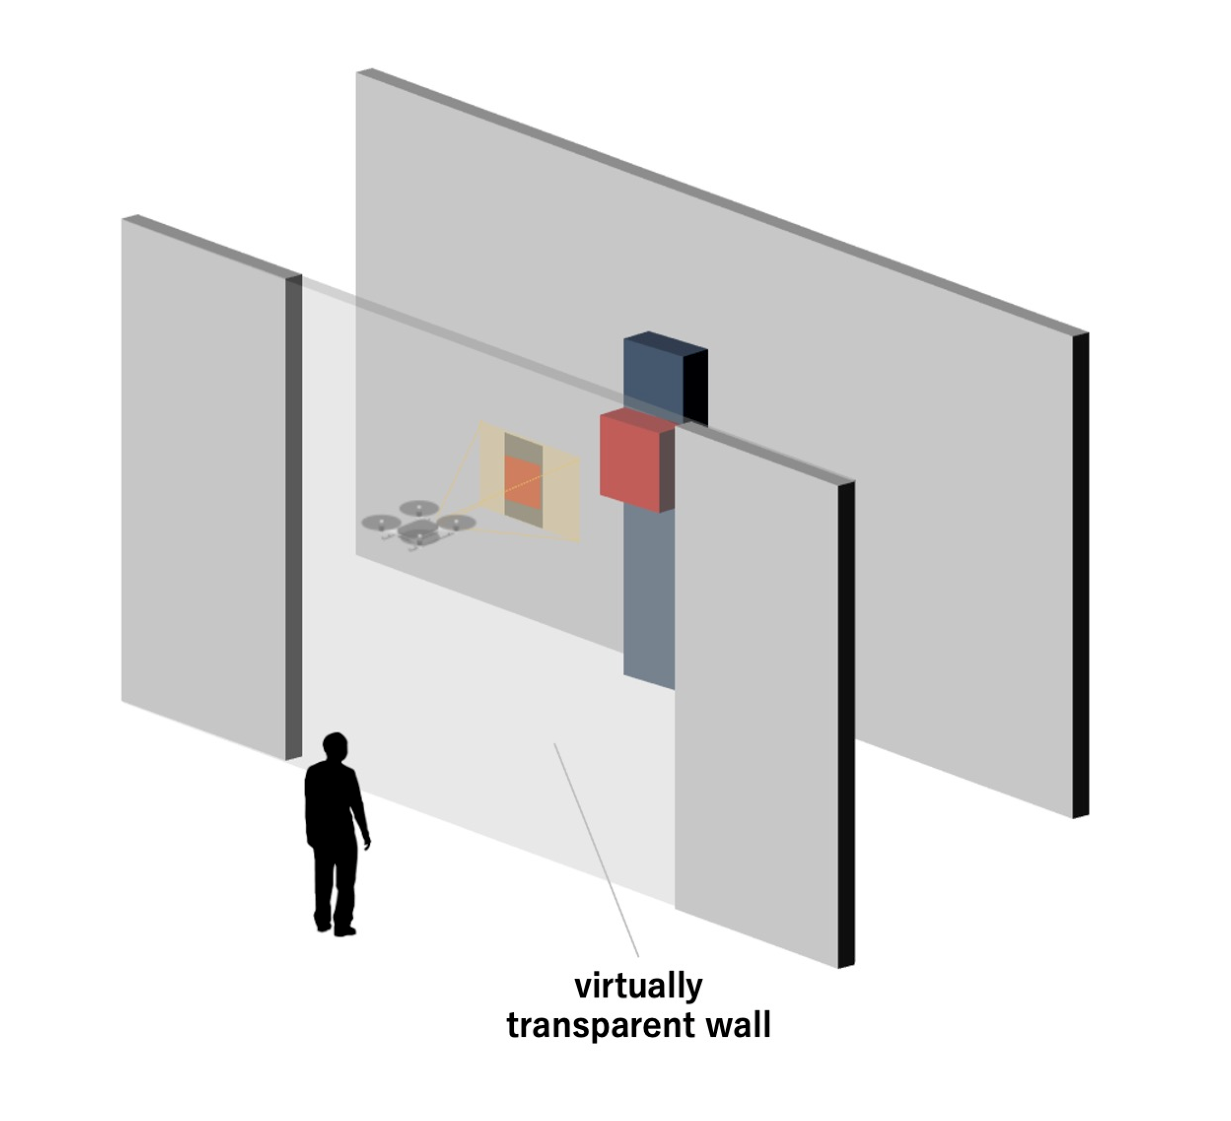
\includegraphics[width=\linewidth]{img/02_relation.eps}
  \caption{死角領域内のAR可視化}
  \ecaption{AR Visualization in the Blind Spot Area.}
  \label{fig:02_relation}
  \end{figure}
  
% -----------------------------------------------------------------  

\par
本研究では,狭小空間による死角領域内のドローン飛行の危険性を軽減するため,Augmented Reality(AR)により操縦者の死角領域内を可視化した一人称視点によるドローン操縦を実現する.
ARは現実の物体の上に,仮想情報を重ねて表示することができるため,この技術を応用する\cite{article-ar03}\cite{article-ar04}.
また,狭小空間では手動によるドローン操縦が求められるため,操縦者にとって障害物回避に有効な情報を確かめるべく,ドローン近傍の障害物を検知するAR方式を提案する.
評価実験は,ドローン操縦の危険性が高い既知の狭小空間探査で行い,狭小空間を素早く,安全に飛行できるか調査した.
探査完了までのドローンの平均操縦時間と,ドローン周辺に位置する障害物への平均衝突警告回数を評価した結果,ARを利用した方式では平均操縦時間,平均衝突警告回数が共に少なかったことから,狭小空間による死角領域内のドローン操縦性向上を示した.
\par
本研究の主な貢献は以下の通りである.
\begin{itemize}
  \item ARと静的な三次元環境地図を利用した,狭小空間監視のためのドローン操縦手法を実現した\cite{article-ar05}.また,実現したドローン操縦手法に加えて,
  ドローン周辺の障害物を知覚するための二種類のAR方式を提案した.
  \item 開発したAR方式の性能を,従来のドローン操縦手法である二人称視点操縦と比較して分析し,狭小空間監視において,どのようなドローン操縦が安全性,操縦性を低減させるか調査した.
  \item 実現した各AR方式を比較して分析し,操縦者へ与える情報量と空間認識能力のトレードオフの調査を行うことで,狭小空間監視におけるドローン操縦にて,操縦者が必要とする情報を示した.
\end{itemize}

% --------------------------- Figure  ---------------------------
\begin{figure}[tb]
  \centering
  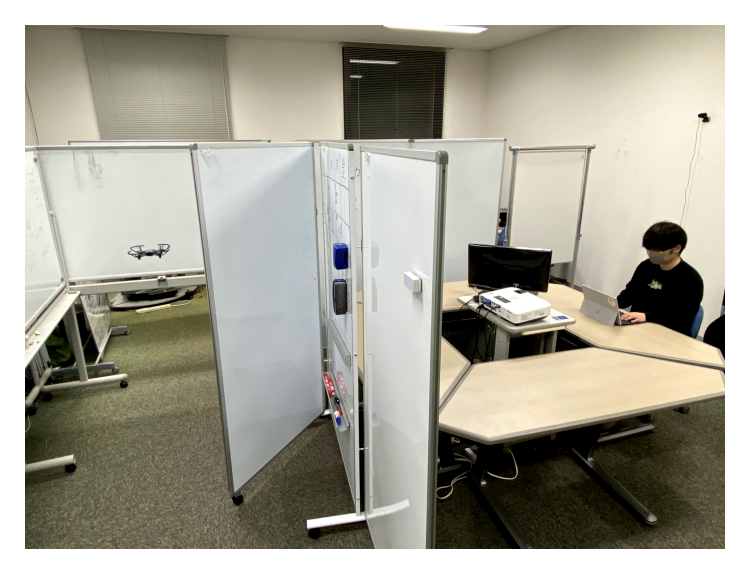
\includegraphics[width=\linewidth]{img/03_enviroment.eps}
  \caption{死角領域内におけるドローン操縦環境}
  \ecaption{Drone Control Environment in the Blind Spot Area.}
  \label{fig:03_enviroment}
  \end{figure}
  
  \begin{figure}[tb]
    \centering
    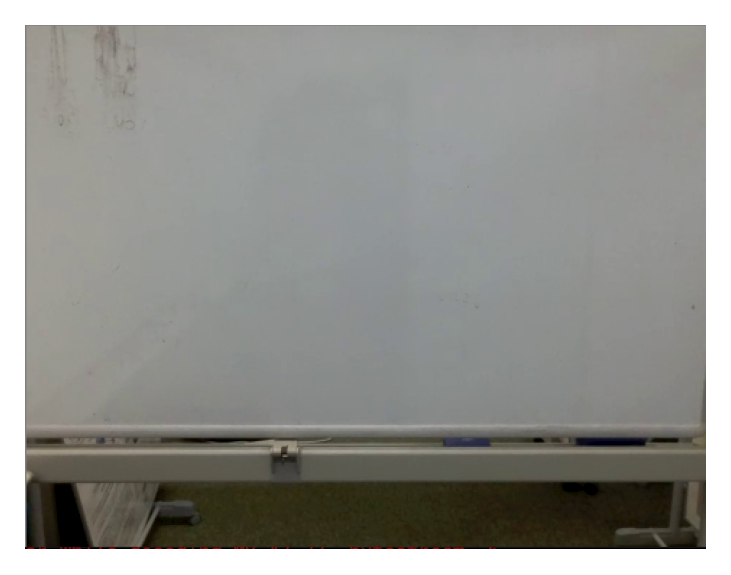
\includegraphics[width=\linewidth]{img/03_fpv.eps}
    \caption{二人称視点方式による操縦画面}
    \ecaption{First-Person View Control Screen.}
    \label{fig:03_FPV}
  \end{figure}
  
  \begin{figure}[tb]
  \centering
  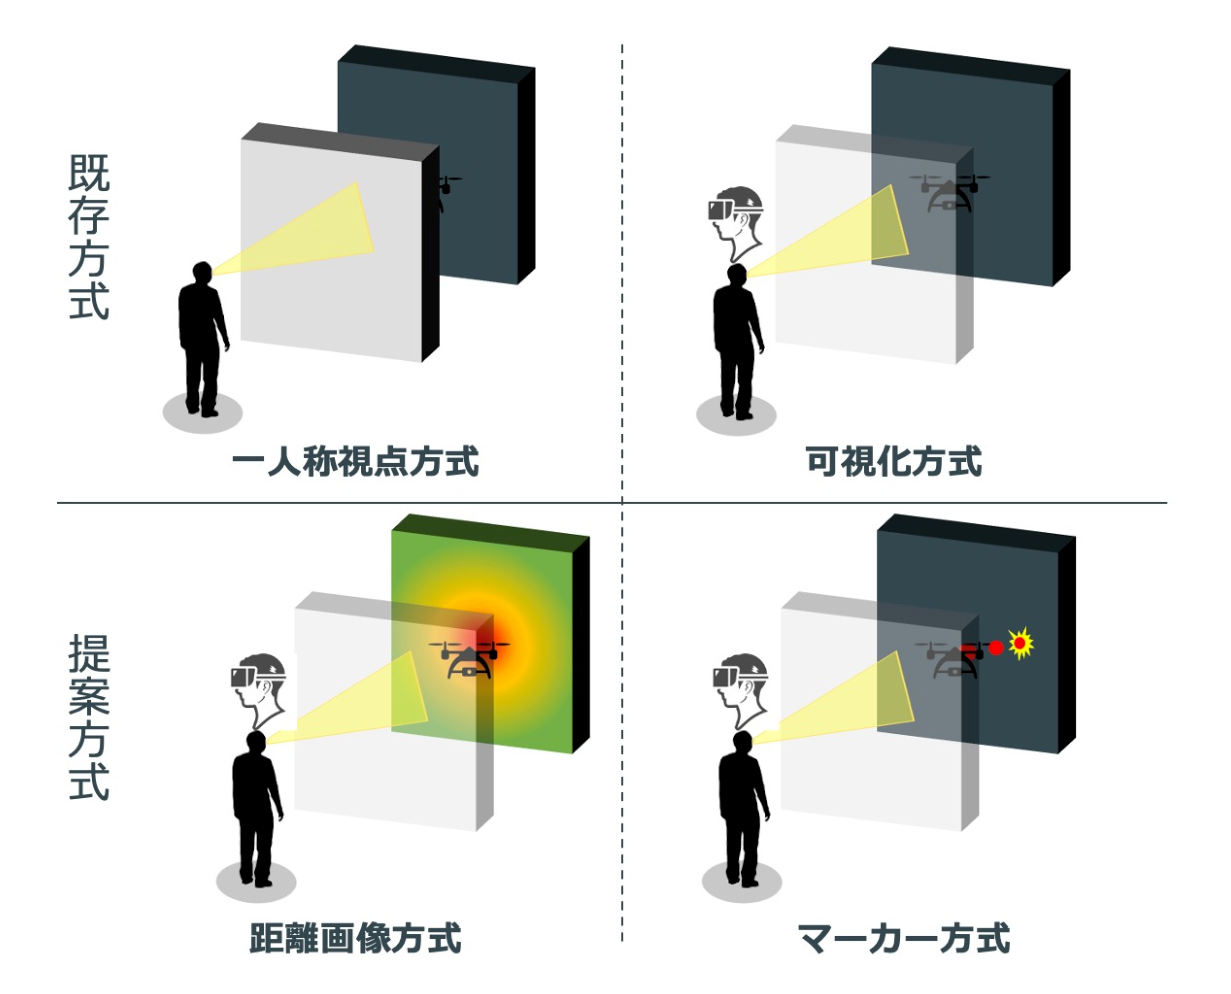
\includegraphics[width=\linewidth]{img/03_outline.eps}
  \caption{提案方式概要}
  \ecaption{Outline of Proposed Method.}
  \label{fig:03_outline}
  \end{figure}
% -----------------------------------------------------------------

%==========================================================================================
%========================================= Section ========================================
%==========================================================================================
\section{関連研究}
\subsection{狭小空間監視でのAR利用の有意性}
Walkerらの研究\cite{book-ar01}では,ARが人間とドローンの相互作用をどのように媒介するかを調査することで,ドローンの意図を視覚的に伝えるための一連の明示的・暗示的なデザインを開発し,ユーザ研究で評価を行った.
その結果,ドローンに対しARを用いたデザインは,ARなしと比べ,課されたタスク効率を大幅に向上させ,ARを用いることでドローンの操縦性を向上させるための,直感的で視覚的な合図を提供できることが示された.

Hedayatiらの研究\cite{book-ar02}では,オンボードカメラ搭載ドローンの撮影した映像を,AR可視化する手法を提案している.結果として,遠隔操作におけるドローン飛行の衝突回数を減少させた.

Kamedaらの研究\cite{book-ar03}では,監視カメラが埋め込まれた場面において,カメラ付きhandy subnotebook PC(HPC)を用いた新しい屋外型複合現実感システムを提案しており,建物や壁などの構造物に隠れて見えない不可視領域の状況を,リアルタイムで可視化できることを示した.

このように,ドローンや死角領域に対してARを用いた関連研究があり,狭小空間による死角領域内のドローン飛行においても適合すると推測する.
また,ARを用いて現実空間に仮想情報を重畳表示することが,効果的であったことを考慮すると,操縦者の見ている現実環境に作用する余地がある二人称視点でのドローン操縦が適していることを示唆している.

% --------------------------- Figure  ---------------------------
  
\begin{figure*}[!tb]
  \centering
  \includegraphics[width=\linewidth]{img/03_comparison.eps}
  \caption{各方式がサポートする機能}
  \ecaption{Functions Supported by Each Method.}
  \label{fig:03_comparison}
\end{figure*}


% -----------------------------------------------------------------

%2.2
\subsection{狭小空間におけるドローン操縦手法}

Liuらの研究\cite{book-ar04}では,ドローン周辺の環境を再構築し,操縦者前方の床やテーブル上に3Dマップを表示することにより,自律航行中のドローンとの直感的なインタラクション手法を提案している.
結果として,操縦者はドローン周辺の三次元環境に没入することができ,飛行空間の探索に成功することができた.
しかし,自律飛行することのできない狭小空間では,操縦者の意図を伝えて飛行させることができない.また,デスクトップPCインタフェースと比較評価した結果,ARインタフェースは操作精度を犠牲にしていた.
そのため,タスク完了までに時間がかかる問題を抱えており,ドローン操縦性を低減する可能性が高い.

Eratらの研究\cite{article-ar05}では,狭小空間による死角領域内の,一人称視点でのドローン操縦手法を提案している.\figref{fig:02_relation}が示すように,事前に空間マッピングにて用意した三次元環境を用いて,閉鎖環境をAR可視化している.
結果として,ドローン視点での二人称視点操縦と比べ,一人称視点でのドローン操縦手法では,タスク完了までの操縦時間が半分以下となっている.

しかし,この関連研究では,ドローン飛行の際に,障害物に衝突しない環境を想定しており,狭小空間での障害物による危険性が提示されていない.
また,二人称視点操縦では,ジョイパッドを用いて操縦していた一方で,一人称視点での操縦では,ハンドジェスチャで操縦していた.
そのため,タスク完了までの操縦時間への有意差が,ARによる空間認識の提供により引き起こされたか明確に述べられていない.そのため,ARにより狭小空間でのドローン操縦性向上が示せるかを確認するため,衝突の危険性を提示し,また,ドローン操縦手法を統一する必要があると考える.

% --------------------------- Figure  ---------------------------

\begin{figure*}[!tb]
  \centering
  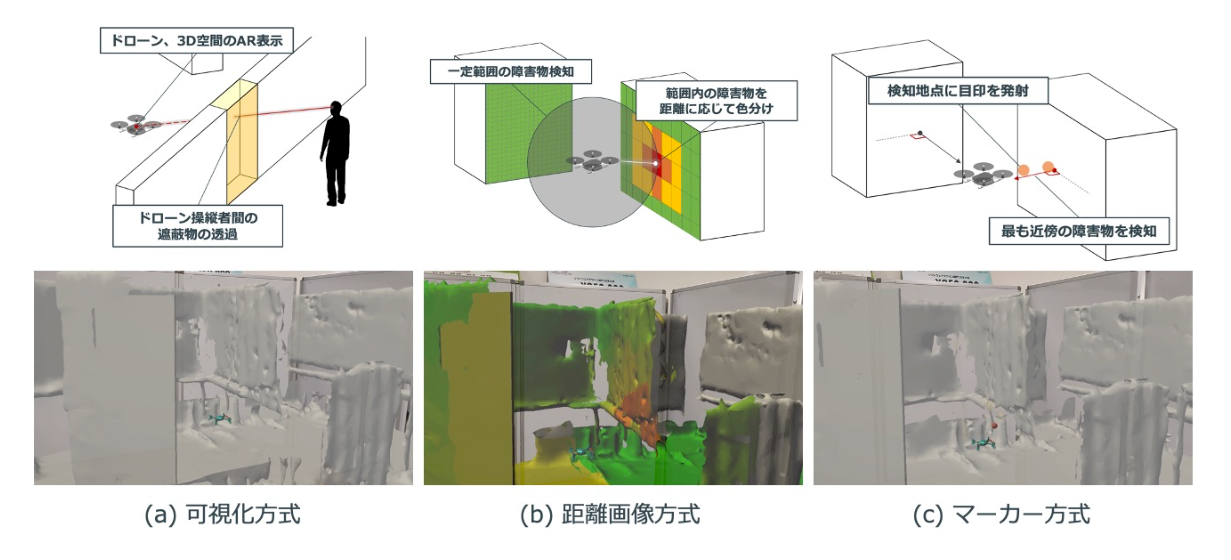
\includegraphics[width=\linewidth]{img/03_preview.eps}
  \caption{各方式の概要および操縦者目線}
  \ecaption{Overview of Each Method and the Pilot's Perspective.}
  \label{fig:03_preview}
\end{figure*}

% -----------------------------------------------------------------

%==========================================================================================
%========================================= Section ========================================
%==========================================================================================

\section{提案方式}
\subsection{概要}
本研究では,狭小空間により,操縦者と小型ドローン(以下,ドローン)の間に遮蔽物があり,ドローンを視認できない環境を「死角領域」とする.\figref{fig:03_enviroment}の環境におけるドローン操縦を想定しており,ARを用いて死角領域内の空間認識を提供し,ドローン周辺の障害物を知覚させることで,ドローン操縦性を向上させる.
\par
先に述べた関連研究\cite{article-ar05}を元に,本研究では2つのドローン操縦手法を用意し,二人称視点方式,可視化方式と呼ぶものとする.
\figref{fig:03_FPV}に示す,ドローンが撮影する映像を頼りに操縦を行う従来のドローン操縦手法である二人称視点方式と,\figref{fig:02_relation}を参考に作成したARを用いて死角領域内の空間認識を提供する可視化方式を比較することにより,関連研究の問題点である死角領域内へのAR適用の有用性を検討する.
また,本研究では可視化方式を元に,ドローン周辺の障害物知覚を支援する2つの方式を提案する.
この2つの方式をここでは,距離画像方式,マーカー方式と呼ぶ.
これら二人称視点方式,可視化方式,距離画像方式,マーカー方式の4つの方式を比較することで,どのような情報が死角領域内のドローン操縦に有効であり,操縦性の向上を示せるか評価する.
各方式の概要を\figref{fig:03_outline},サポートしている機能を\figref{fig:03_comparison}に示す.
また\figref{fig:03_preview}に,可視化方式,距離画像方式,マーカー方式の3つの方式の操縦者目線を示す.

\subsection{可視化方式}
可視化方式では,ドローンと操縦者の間に遮蔽物が存在する場合,ドローンが飛行している場所が操縦者にとっての死角領域となる.
死角領域が存在すると判断したとき,事前に空間マッピングした三次元環境地図における遮蔽物を透過した上で,現実環境に重畳表示することで,仮想的に死角領域の空間認識を提供する.操縦者は,死角領域内を飛行するドローンを視認することはできないが,ARによって仮想のドローンと,ドローン周辺の三次元環境を視認することができる.
\par
\figref{fig:03_preview}左のように,遮蔽物によって視認できないドローンと,そのドローン周辺の環境をARによって可視化している.障害物を知覚せず,可視化による空間認識の視覚支援のみを行なっている.


\subsection{距離画像方式}
距離画像方式は,ステレオビジョンを参考にして,ドローンから障害物までの距離に応じて,障害物の色を分けている.障害物を3色に分類することで,近傍の障害物の危険性を警告する.
距離画像方式は,全体的な環境の理解を提供しており,ドローン周辺の障害物に対する衝突の危険性を示す.
\par
距離画像方式では,障害物までの危険な距離を閾値a,未だ猶予はあるが慎重に動くべき距離を閾値bとする.
常に周りの障害物までの距離を計測し,閾値を元に以下のいずれかの動作をする.

\begin{enumerate}
	\item ドローンからの距離が閾値a 未満の障害物を赤色に変更
    
  \item ドローンからの距離が閾値a 以上 〜 閾値b 未満の障害物を赤色から黄色に変更
    
  \item ドローンからの距離が閾値b 以上の障害物を緑色に変更
\end{enumerate}

\figref{fig:03_preview}中央のように,ドローン本体ではなく,ドローン周辺の環境を拡張しており,ドローン周辺の障害物の危険度を理解できる,色彩の変化による視覚支援を行なっている.赤色に変化した障害物の方向には衝突の危険性,黄色になっている障害物の方向には慎重な操縦の必要性,一方で緑色の障害物の方向には進んでも衝突の危険性がないことを示し,操縦者への安心感を提供する障害物知覚を行っている.



\subsection{マーカー方式}
マーカー方式は,ドローンから見て最も近い障害物に対して,障害物までの距離に応じて,色分けを行なった目印を付けている.距離画像方式では障害物すべてが色分けされているため,操縦者を混乱させる可能性がある.マーカー方式では,選択的注意を参考に,最も危険な障害物のみを知覚させるため,距離画像方式に比べ簡易的なアプローチとなっている.
\par
マーカー方式では,障害物までの危険な距離を閾値a,未だ猶予はあるが慎重に動くべき距離を閾値bとする.
常に周りの障害物までの距離を計測し,閾値を元に以下のいずれかの動作をする.

\begin{enumerate}
	\item ドローンからの距離が閾値a 未満の最も近傍の障害物に対して赤色の目印を示す
    
    \item ドローンからの距離が閾値a 以上 〜 閾値b 未満の最も近傍の障害物に対して黄色の目印を示す
\end{enumerate}

\figref{fig:03_preview}右のように,ドローン自体を拡張しており,どの障害物が危険か一目で理解できる,直感的視覚支援を行なっている.赤色の目印が向けられている障害物はこれ以上進むと衝突の危険性があり,黄色の目印が向けられている障害物は慎重な操縦を求め,操縦者への危機感を与える視覚的支援を行なっている.

% --------------------------- Figure  ---------------------------

\begin{figure}[tb]
  \centering
  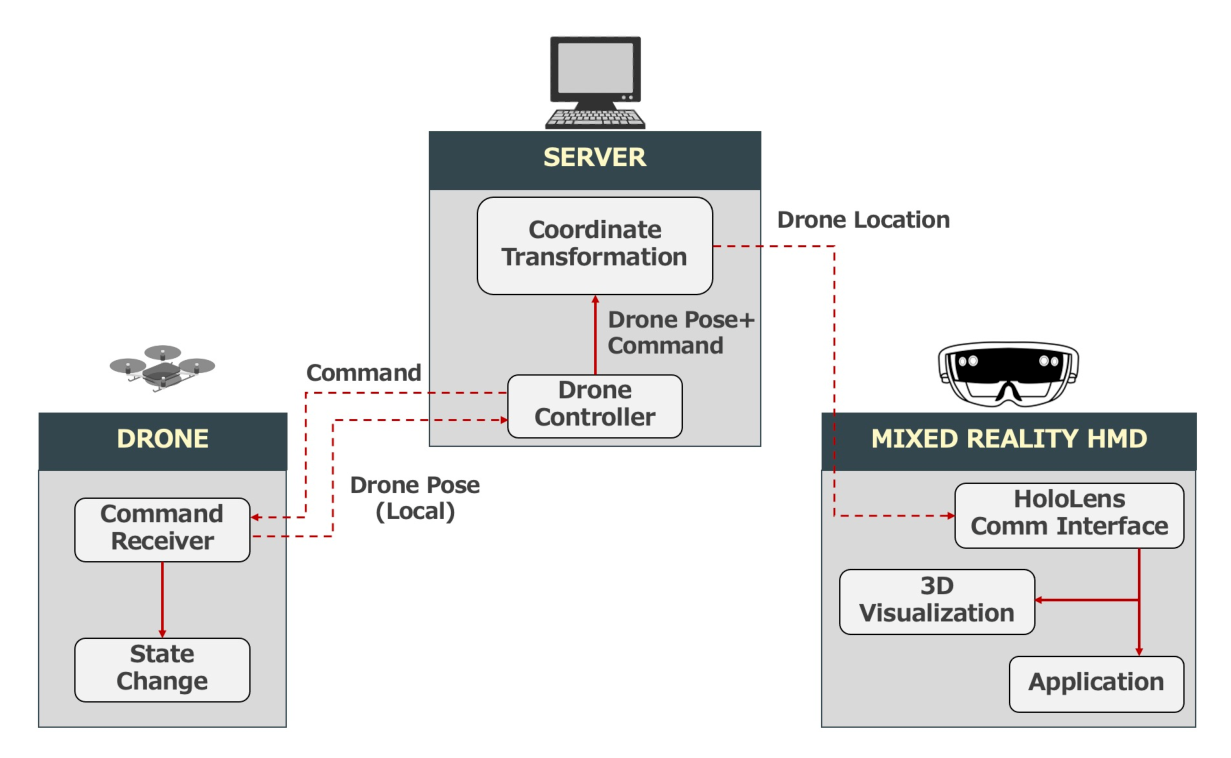
\includegraphics[width=\linewidth]{img/04_system.eps}
  \caption{システム構成}
  \ecaption{System Configuration.}
  \label{fig:04_system}
\end{figure}
  
% -----------------------------------------------------------------

%==========================================================================================
%========================================= Section ========================================
%==========================================================================================
\section{評価}

\subsection{実装環境}
本研究で開発したシステム構成を\figref{fig:04_system}に示す.
実際に使用したドローンはRyze Tech社製Tello EDU(以下,Tello)であり,操作端末はMacBookProを用いる.Telloはプログラミングによってフライトコントロールを行うことができ,規定のコマンドを送信することで飛行制御することができる.
\par
ARHMDはMicrosoft HoloLens2(以下,HoloLens)を使用する.
事前に,HoloLensのSpatial Mappingにより空間マッピングを行うことで空間のメッシュデータを入手し,静的な三次元環境地図を作成する.
作成した三次元環境地図を,ゲーム・アニメーションエンジンであるUnity内の3D仮想空間上に配置し,操縦者の位置情報と,Unity内の三次元環境地図の位置合わせを行うことで,空間認識を提供する.
\par
サーバではTello,HoloLensとUDP通信\cite{web-udp}を行なっており,常時,Telloの傾きや移動距離をHoloLensに送信する.
Telloより受け取った値をUnity 座標系へ変換し,変換後の値を反映させることにより,仮想ドローンの位置合わせを行っている.
ここでUDPを使用する理由として,Tello,サーバ,HoloLens間の遅延低減を目的とする.
\par
距離画像方式,マーカー方式では,共に障害物までの距離によって,危険度を色で示している.操縦者がドローンを操縦するとき,衝突する危険性がある距離を0.3m とし\cite{tech-01},距離画像方式では,障害物までの距離が0.3m までを赤色,0.3m 〜 0.6m までを黄色,0.6m 以上を緑色で示す.マーカー方式では障害物までの距離が0.3m までを赤色の目印,0.3m 〜 0.6m の際に黄色の目印を示す.

\subsection{タスク}
実験環境は\figref{fig:04_experiment}に示すように,スタート地点,障害物,ゴール地点で構成されており,実験参加者は,ドローンをスタート地点から目的地まで操縦し,目的地で着陸するタスクを行った.その間,上下左右に移動しなければ衝突の恐れがある障害物を設置した.\figref{fig:04_experiment}に赤色で示されている障害物を回避する必要があり,避けなければ通過が困難になるよう設定している.実際の狭小空間では,速さではなく,衝突のない安全飛行が必要であるため,参加者にはタスクの早期終了ではなく,障害物にぶつかることなく,慎重に通過することを要求した.実験では二人称視点方式,可視化方式,距離画像方式,マーカー方式の計4つの方式を用いた.ARを用いた方式では,ドローンの進行方向を分かりやすくするため,ドローン前方を赤色で示している.

% --------------------------- Figure  ---------------------------
\begin{figure}[tb]
  \centering
  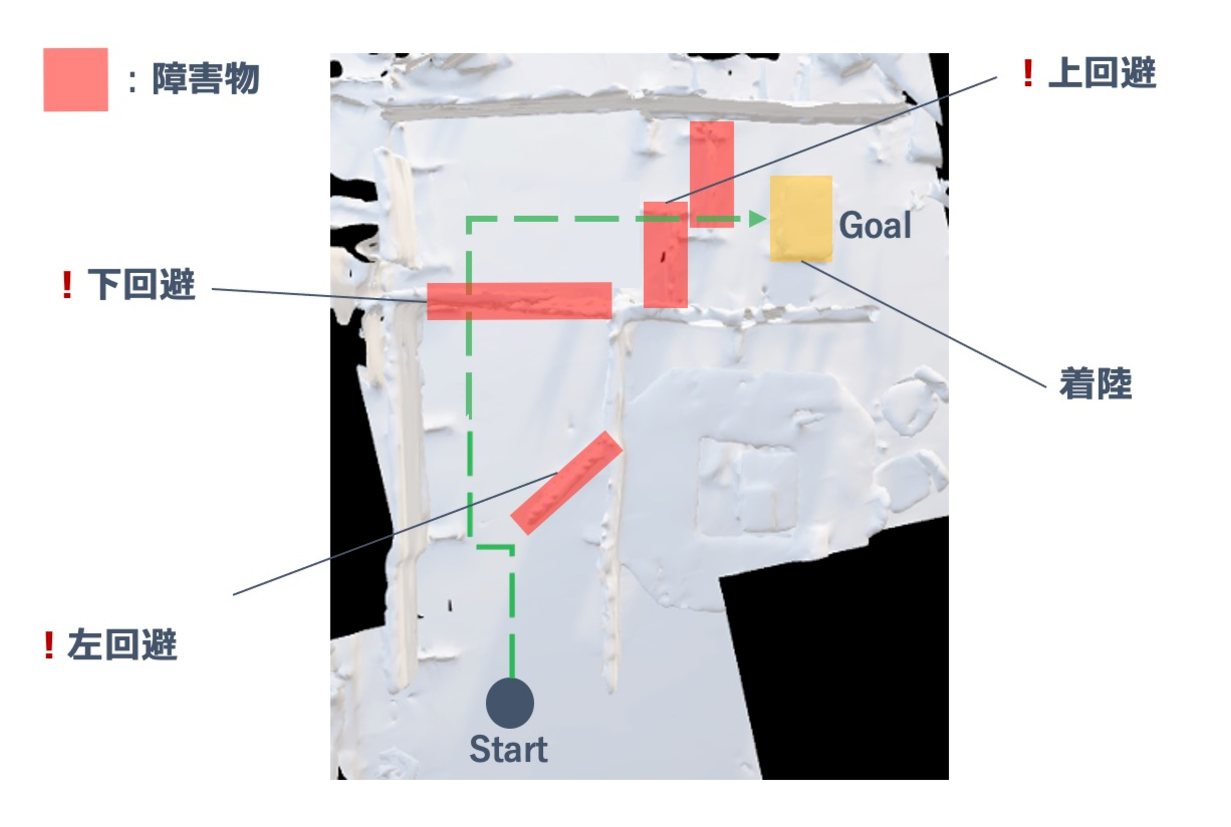
\includegraphics[width=\linewidth]{img/04_experiment.eps}
  \caption{実験環境}
  \ecaption{Experimental Environment.}
  \label{fig:04_experiment}
\end{figure}
% -----------------------------------------------------------------

\subsection{評価実験}
死角領域内を飛行するドローンの操縦において,各方式がどのような影響を与えるかを評価するため,10人の実験協力者による実験を行なった.
参加者の平均年齢は22歳であり,ドローン操縦経験はなかった.
実験は約60分で行い,導入,各提案方式の練習,ARのキャリブレーション,タスク,アンケートの5つのフェーズから構成する.
まず,参加者は本研究の概要と,操縦方法の説明を受け,その後,各方式の練習を行う.予備実験で,操縦の慣れによる実験後半の操縦時間短縮や,ARの経験がないことによる操縦時間増加を引き起こすことがわかった.
そのため,この効果を打ち消すために,ドローン操縦を5〜10分ほど練習した後に,各方式で実験環境を1度飛行することで,練習量を増やし,慣れによる差異を無くした.
次にAR方式では,HoloLensアプリケーションを起動し,現実空間とのキャリブレーションを行い,参加者はHoloLensを装着した.
その後,タスクを行い,各方式でタスクを完了する度に,実験を行なった方式についてアンケートを記入し,全方式を終了したら,どの方式が最も効果的であったかを選択し,その理由を記入してもらった.
また,なぜ他の方式を選択しなかったのか,その理由も記入してもらった.

\subsection{評価項目}
提案方式の有効性を評価するにあたり,ドローン技術の熟練度による差を出さないために,Telloの速度,一度に進む距離,旋回角度は事前に設定している.またサーバのスペック,サーバよりTelloへ送信するコマンドのパラメータの設定を\tabref{tab:server_spec},\tabref{tab:command_parameter}に示す.
狭小空間監視では,衝突することのできない点検や,迅速な対応が求められる災害現場など,ドローンを素早く,安全に操縦することが求められる.
そのため,各方式における,操縦者がタスクを完了するまでの操縦時間,障害物への衝突警告回数の2項目による客観的な評価と,参加者へのアンケート,自由回答による主観的な評価を記録した.
障害物の衝突警告回数では,実際に衝突してしまう恐れがあるため,操縦者がドローンを進行させようとしている方向に存在する障害物との距離を計測し,距離が0.3 m以内の際に操縦者へ警告がされるようになっている.
\tabref{tab:command_parameter}に示すように,ドローンの進行距離を0.3 mとしているため,衝突警告距離の閾値を0.3 mとした.
また参加者へのアンケートでは,主観的な認識と好みを測定するために,7ポイントのリッカート尺度のアンケートを実施した.
アンケートでは二人称視点方式とARを利用した3つの各方式を比較できるように実施し,また,AR同士での比較が行えるように,ARを用いた方式のみ別途アンケートを実施した.
二人称視点方式とARを用いた3つの各方式を比較するアンケートでは,操縦の安心度,危険な障害物を判断できたかの2項目を設けた.
また,ARを用いた方式のみを比較するアンケートでは,状況把握の容易さ,操縦の自信度の2項目を設けた.
実験の最後には,参加者にはどの方式が最も操縦性が良かったかを選択し,なぜその方式が良かったのか,また,なぜ他の方式を選択しなかったかという項目を設けた.タスク完了までの平均操縦時間には一次元配置分散分析(one-way analysis of variance:以下,ANOVA)を用いて統計解析した.また,Post-hoc検定では,Tukey’s Honestly Significant Difference(Tukey HSD)検定を行い,各方式の比較を行なった.平均衝突警告回数,アンケート結果では,Friedman検定を行い,Post-hoc検定ではBonferroni法を行い,各方式の比較を行なった.

% --------------------------- Figure  ---------------------------


\begin{table}[tb] 
  \caption{サーバの性能} 
  \ecaption{Server Performance.}
  \label{tab:server_spec}
  \hbox to\hsize{\hfil
  \begin{tabular}{cc}\hline\hline
  OS & macOS 11.0.1 \\
  CPU & 2.4 GHz Intel Core i4 \\
  メモリ & 8 GB \\
  使用言語 & Python 2.7 \\ \hline
  \end{tabular}\hfil}
\end{table}


\begin{table}[tb] 
  \caption{ドローンへ送信するコマンドのパラメータ} 
  \ecaption{Parameters of the Command to Be Sent to the Drone.}
  \label{tab:command_parameter}
  \hbox to\hsize{\hfil
  \begin{tabular}{cc}\hline\hline
  命令コマンド & パラメータ \\ \hline
  前進後退 & 0.3 m \\
  左右移動 & 0.3 m \\
  上昇下降 & 0.3 m \\
  左右旋回 & 20 度 \\
  送信間隔 & 0.3 m \\ \hline
  \end{tabular}\hfil}
\end{table}

\begin{figure}[tb]
\centering
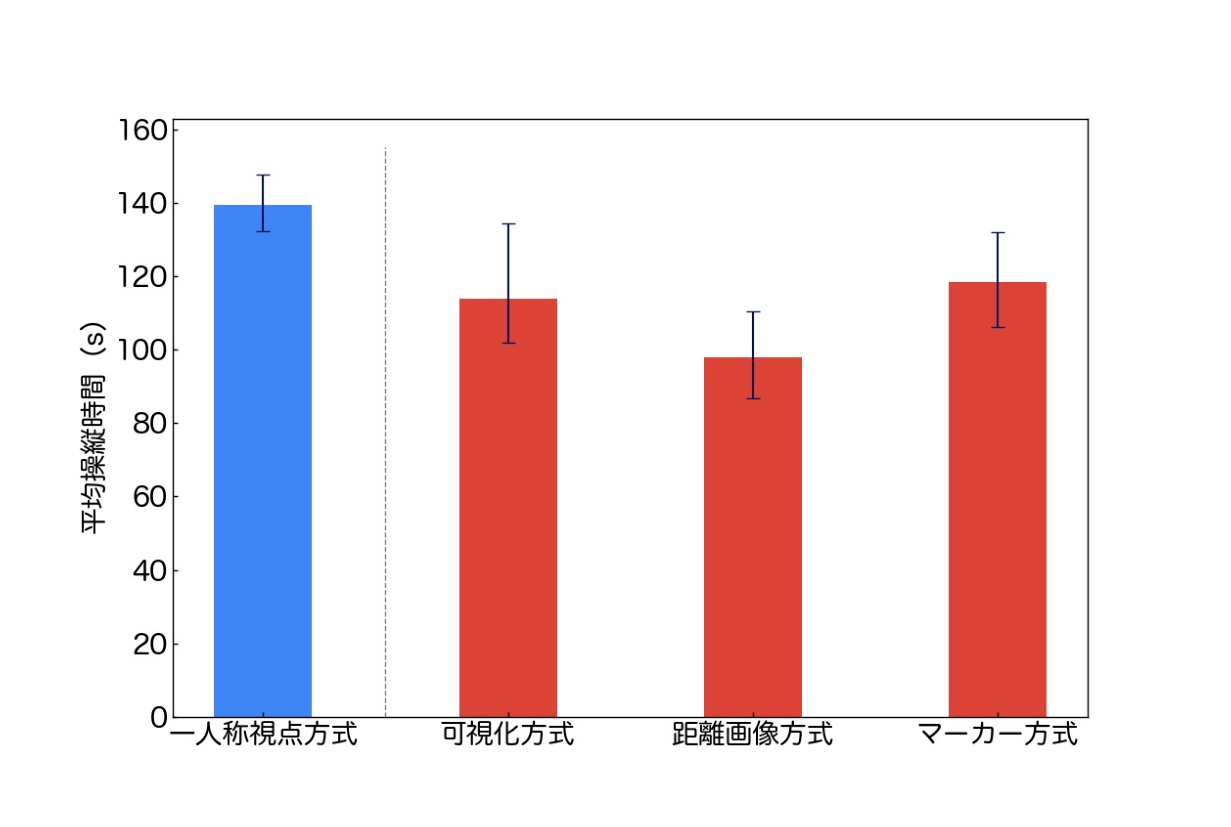
\includegraphics[width=\linewidth]{img/04_bar1.eps}
\caption{平均操縦時間}
\ecaption{Average Maneuvering Time.}
\label{fig:04_bar1}
\end{figure}

\begin{figure}[tb]
\centering
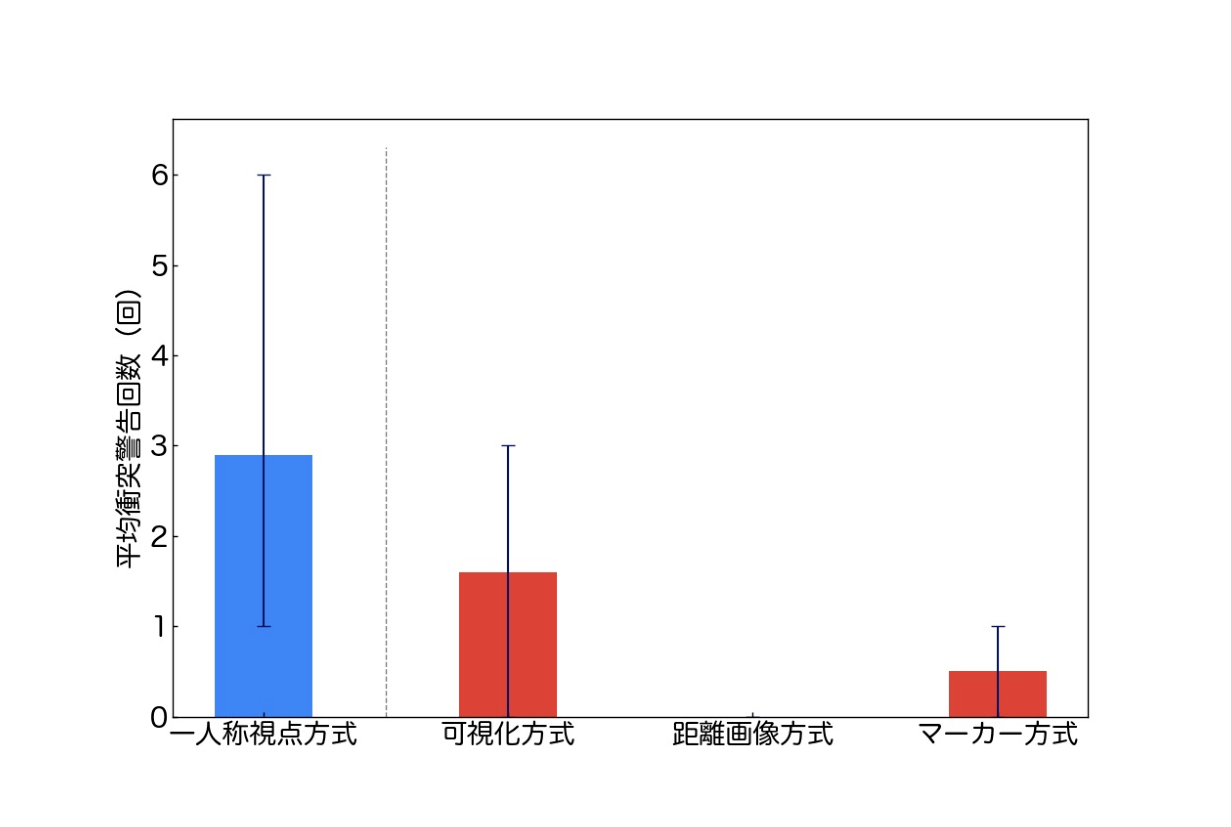
\includegraphics[width=\linewidth]{img/04_bar2.eps}
\caption{平均衝突警告回数}
\ecaption{Average Number of Collision Warnings.}
\label{fig:04_bar2}
\end{figure}

% -----------------------------------------------------------------

\subsection{ドローン操縦の定量的評価}
\label{result_1}
タスク完了までの平均操縦時間の評価結果を\figref{fig:04_bar1}に示す.
平均操縦時間では,ANOVAの結果,4群間に有意差を示した($F$(3,36) = 48.35, $p = 1.04e-12 $).Tukey HSD検定を用いた多重比較($p < 0.05$)では,二人称視点方式とARを用いた各方式を比較した場合,可視化方式($p < 0.001$),距離画像方式($p < 0.001$),マーカー方式($p < 0.001$)となり,平均操縦時間は有意に減少することがわかった.
ARを用いた方式同士では,距離画像方式と各方式を比較した場合,可視化方式($p < 0.001$),マーカー方式($p < 0.001$)となり,有意に操縦時間が減少したことがわかった.しかし,可視化方式とマーカー方式の間では,有意にタスク完了時間が減少しないことがわかった($p = 0.545$).
\par
次に,障害物への平均衝突警告回数の結果を\figref{fig:04_bar2}に示す.平均衝突警告回数では,Friedman検定の結果,4群間に有意差を示した($\chi^{2}(3)=24.307, p < 0.001$).
Bonferroni法の多重比較($p < 0.05$)では,二人称視点方式とマーカー方式($p < 0.05$),距離画像方式($p < 0.05$)の間には有意差を示したが,可視化方式との間では有意差は示さなかった($p = 0.163$).
ARを用いた方式同士では,可視化方式と各方式を比較した場合,マーカー方式との間には有意差を示さなかったが($p = 0.069$),距離画像方式との間には有意差を示した($p < 0.05$).
しかし,距離画像方式とマーカー方式間では,有意差を示さなかった($p = 1.000$).

% --------------------------- Figure  ---------------------------

\begin{figure}[tb]
  \centering
  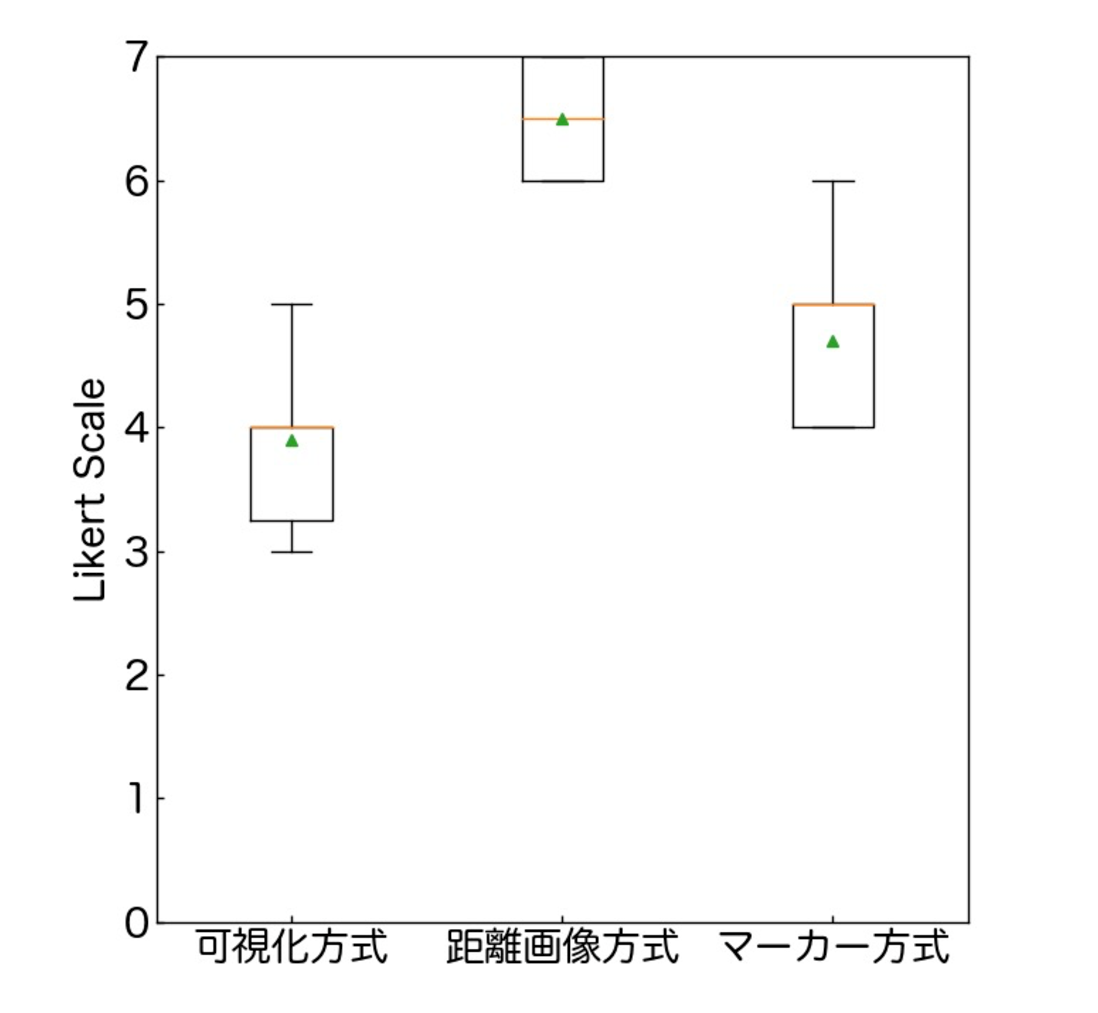
\includegraphics[width=\linewidth]{img/04_likert1.eps}
  \caption{操縦の安心度}
  \ecaption{Level of Security of Operation.}
  \label{fig:04_likert1}
  \end{figure}
  
  % -----------------------------------------------------------------

\subsection{ドローン操縦の定性的評価}
\label{result_2}
二人称視点方式とARを用いた3つの各方式を比較するアンケート結果を\figref{fig:04_likert1},\figref{fig:04_likert2}に示す.
二人称視点方式を含むアンケート結果では,操縦の安心度($\chi^{2}(3)=27.875, p < 0.001$),危険な障害物知覚($\chi^{2}(3)=28.372, p < 0.001$)の2項目に対してFriedman検定を行ったところ,有意差を示した.
それぞれの結果に対しBonferroni法の多重比較($p < 0.05$)を行ったところ,操縦の安心度では,二人称視点方式とマーカー方式,距離画像方式間に有意差を示した($p < 0.05$)が,可視化方式との間には有意差を示さなかった($p = 0.076$).
また,可視化方式とマーカー方式間には有意差を示さなかった($p = 0.251$)が,距離画像方式は可視化方式,マーカー方式との間にも有意差を示した($p < 0.05$).
危険な障害物を判断できたかを確認する項目では,二人称視点方式と距離画像方式,マーカー方式間に有意差を示した($p < 0.05$)が,可視化方式との間には有意差を示さなかった($p = 0.124$).
また,可視化方式とマーカー方式間には有意差を示さなかった($p = 0.107$)が,距離画像方式は可視化方式,マーカー方式との間にも有意差を示した($p < 0.05$).
\par
次に,ARを用いた方式のみを比較するアンケート結果を\figref{fig:04_likert3},\figref{fig:04_likert4}に示す.
ARを用いた方式のみを比較するアンケート結果では,状況把握の容易さ($\chi^{2}(2)=18.667, p < 0.001$),操縦の自信度($\chi^{2}(2)=17.886, p < 0.001$)の2項目に対してFriedman検定を行ったところ,有意差を示した.
それぞれの結果に対しBonferroni法の多重比較($p < 0.05$)を行ったところ,
状況把握の容易さでは,可視化方式とマーカー方式間には有意差を示さなかった($p = 0.091$)が,距離画像方式のみ可視化方式とマーカー方式の間に有意差を示した($p < 0.05$).
操縦の自信度でも同じく,可視化方式とマーカー方式間には有意差を示さなかった($p = 0.059$)が,距離画像方式のみ可視化方式とマーカー方式の間に有意差を示した($p < 0.05$).

% --------------------------- Figure  ---------------------------

\begin{figure}[tb]
\centering
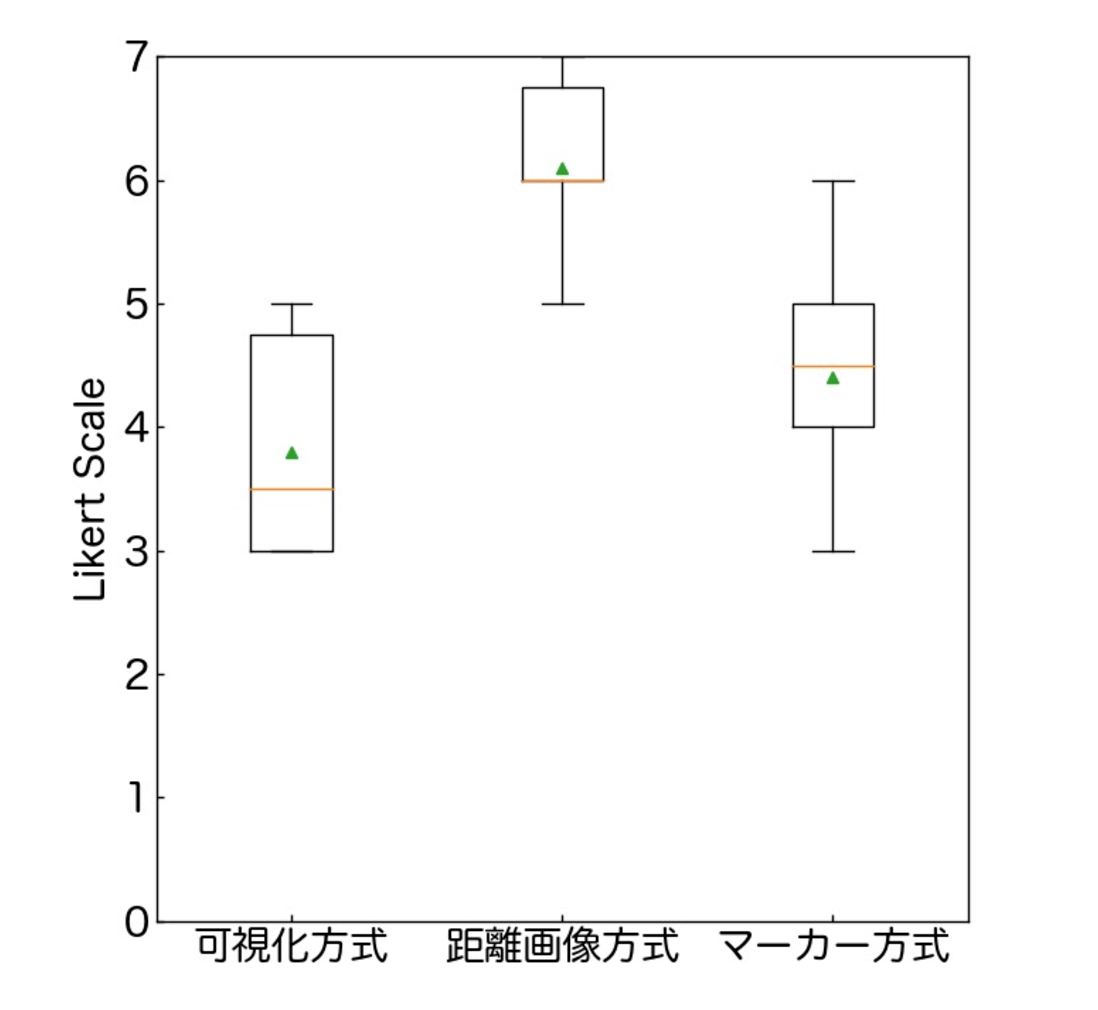
\includegraphics[width=\linewidth]{img/04_likert2.eps}
\caption{危険な障害物を判断できたか}
\ecaption{Dangerous Obstacle Perception.}
\label{fig:04_likert2}
\end{figure}

% -----------------------------------------------------------------



%==========================================================================================
%========================================= Section ========================================
%==========================================================================================

\section{考察}
\subsection{AR方式の有用性}
ARを用いた方式は,\ref{result_1}節で述べたように,二人称視点方式に対して有意差を示した.
タスク完了までの平均操縦時間では,ARを用いた方式は全て,二人称視点方式と比較して有意に時間が減少している.
実験の様子から,二人称視点方式では周囲に何があるか分からず,確認する動作が他方式に比べ多くなるため,操縦時間が増大していた.
本研究で想定しているようなドローンは最大飛行時間が短いことが問題点とされている中で\cite{article-drone14}\cite{article-drone15}\cite{article-drone16},距離画像方式では,従来の操縦手法である二人称視点方式の操縦時間と比較して約30\% 減少しているため,作業効率の向上が見込める.
また二人称視点方式は,タスク完了までの平均操縦時間と,平均衝突警告回数より,1分間の間だけで約1.25回も衝突の可能性があり,実際の狭小空間における操縦手法として危険性が高いことを確認した.
\par
障害物への平均衝突警告回数では,ARを用いた方式の中でも,可視化方式は二人称視点方式との間に有意差を示さなかった.
しかし,距離画像方式やマーカー方式のような障害物を知覚するための方式では,二人称視点方式との間において,平均操縦時間,平均衝突警告回数共に有意差を示していた.
また,\ref{result_2}節で述べた,主観的結果における二人称視点方式とAR方式の比較結果では,二人称視点方式と可視化方式間には有意差を示さなかった.
このことより,狭小空間による死角領域内を可視化するだけでは,一人称視点でドローン操縦を行なっていても,障害物へ衝突する危険性や,操縦者に与える心理的負荷を低減することは困難である.
そのため,ARを用いた死角領域内の可視化だけでなく,ドローン周辺の障害物に対する視覚的支援を行う本提案方式では,ドローン操縦性向上を示せることがわかった.

% --------------------------- Figure  ---------------------------

\begin{figure}[tb]
  \centering
  \includegraphics[width=\linewidth]{img/04_likert3.eps}
  \caption{状況把握の容易さ}
  \ecaption{Ease of Understanding the Situation.}
  \label{fig:04_likert3}
  \end{figure}

% -----------------------------------------------------------------

\subsection{AR方式の比較}
\subsubsection{定量的評価}
\ref{result_1}節で述べた,客観的結果におけるAR方式同士の有意差について考察する.
タスク完了までの平均操縦時間では,可視化方式とマーカー方式の間で有意差を示さなかった.
実験参加者の自由回答では,マーカー方式では,操縦の際に躊躇ってしまう傾向があり,また,
可視化方式では,操縦の際に思い切って進む傾向があった.
このことから,マーカー方式では1箇所のみ危険な場所に目印を付けているため,操縦に躊躇いが生じ,慎重になり,
その一方で,可視化方式では,どこの障害物が危険か判断できず,思い切って操縦するためことが推測される.
そのため,マーカー方式では可視化方式と比べ,操縦時間が長くなっていることがわかる.
\par
障害物への平均衝突警告回数では,二人称視点方式と可視化方式との間では有意差を示さなかった.
その一方で,距離画像方式,マーカー方式は二人称視点方式との間に有意差を示しているため,ドローン周辺の障害物との距離感が掴めない問題を解消できていると推測される.
また,距離画像方式とマーカー方式の間では有意差を示さなかった.
しかし,実際にドローン操縦を行う際にドローンの衝突は0に収めなければならないことを考えると,距離画像方式では平均衝突警告回数を0回に収めたことより,有意な結果であると考察できる.

\subsubsection{定性的評価}
\ref{result_2}節で述べた,主観的結果におけるAR方式同士の有意差について考察する.
\figref{fig:04_likert3},\figref{fig:04_likert4}で示すアンケート結果では,可視化方式とマーカー方式の間において,一貫して有意差を示さなかった.
実験参加者の自由回答では,マーカー方式では,気になる障害物に対して目印を示さない傾向があった.
このことから,ドローン周辺に衝突の可能性のある障害物が2つ以上ある際に,操縦者が手に入れたい障害物までの距離感を示さない可能性があるため,可視化方式と比べ有意差を示さなかったと考察できる.

% --------------------------- Figure  ---------------------------

\begin{figure}[tb]
\centering
\includegraphics[width=\linewidth]{img/04_likert4.eps}
\caption{操縦の自信度}
\ecaption{Confidence in Piloting.}
\label{fig:04_likert4}
\end{figure}

% -----------------------------------------------------------------

\subsection{統合的評価}
実験の終了後にどの方式が最も効果的であったかを実験参加者に選択してもらった結果,9名が距離画像方式を選択し,1名がマーカー方式を選択した.
距離画像方式を選択した理由として,障害物までの距離を色で示していることによって距離感を掴みやすかった点や,見える景色全体に色がついているため,どの範囲まで動かすことができるか分かりやすかった点が挙げられた.
一方で,他の方式を選択しなかった理由として,二人称視点方式では,上下の障害物までの距離感が掴づらかった点や,周囲の確認に不安があった点が挙げられた.
可視化方式では,全体像は掴めたが状況認識が難しかった点や,距離感に自信を持てない点が挙げられ,マーカー方式では,一方向でしか距離感が分からなかった点が挙げられた.
一方でマーカー方式を選択した参加者は,最も近傍の障害物を示してくれる安心感がある点からマーカー方式を選択し,距離画像方式では周囲が赤色になった際に困惑した点や,見えている情報が簡潔でない点から選択しなかった.
以上のことから,死角領域内を可視化するだけでは狭小空間のドローン操縦は不十分である.狭小空間でのドローン操縦では,死角領域内を可視化に加えて障害物知覚が必要であり,操縦者にとって重要な情報は,最も危ない位置を示すような直感的な情報ではなく,常に周囲の危険性を示す全体的な把握を促せる情報であることがわかった.
周辺環境の全体的な理解と安心感を提供する距離画像方式では,\figref{fig:04_bar1},\figref{fig:04_bar2}に示すように,他の方式と比べ平均操縦時間の減少,衝突回数の減少を可能にすることができたため,狭小空間による死角領域内の環境下において,ドローン操縦性向上に有効であることを確認した.

%==========================================================================================
%========================================= Section ========================================
%==========================================================================================
\section{まとめ}
\label{sec:Conclusion}
小型ドローンは機体の大きさを活かして,インフラ点検や災害調査のような,人間が立ち入れない狭小空間での活躍が増えている.しかし,狭小空間でのドローン飛行では,遮蔽物により視点が遮られる,死角領域内での操縦を必要とする.また,従来の操縦手法では状況認識が不十分であるため,ドローン周辺に位置する障害物が多い狭小空間では,ドローン操縦は困難である.\par
遮蔽物,障害物が多い狭小空間では,死角領域内におけるドローン飛行の危険性を軽減する必要がある.
そこで本研究では,ARにより操縦者の死角領域内に存在するドローンと周辺環境を可視化し,ドローン周辺の障害物を知覚するためのAR方式を提案する.
本提案方式について,死角領域内でのドローン操縦性を評価実験した.
結果として,ARを利用した方式では実験環境での平均操縦時間が短く,平均衝突警告回数も少なかったことから,狭小空間による死角領域内のドローン操縦性向上を示した.
また,障害物を知覚するためのAR方式では,ドローン周辺の障害物に対し,危険度を色で振り分けている方式が操縦者へ安心感を与え,操縦性が向上することを確認した.

%==========================================================================================
%========================================= Section ========================================
%==========================================================================================
\bibliography{bibliography}

%==========================================================================================
%========================================= Section ========================================
%==========================================================================================
\begin{biography}
\profile{s}{竹内 一真}{2021年同志社大学理工学部情報システムデザイン学科卒業.同年同志社大学大学院理工学研究科情報工学専攻修士課程進学.}
%
\profile{n}{滕 睿}{2006年東京大学情報理工学系研究科博士後期課程修了.2021年より同志社大学モビリティ研究センター.V2Xネットワーク,IoT等の研究に従事.電子情報通信学会,IEEE各会員.}
%
\profile{m}{佐藤 健哉}{同志社大学大学院理工学研究科情報工学専攻教授.1986年大阪大学大学院工学研究科電子工学専攻修士課程修了.同年住友電気工業情報電子研究所入社.1991〜1994年スタンフォード大学計算機科学科客員研究員.2000年奈良先端科学技術大学院大学情報科学研究科博士後期課程修了.米国AMI-C,Inc. チーフテクノロジストを経て,2004年より現職.同志社大学モビリティ研究センター長,および名古屋大学大学院情報学研究科附属組込みシステム研究センター特任教授兼務.博士(工学).IEEE-CS,ACM,自動車技術会各会員.}
\end{biography}

\end{document}
